\documentclass[11pt]{article}
\usepackage{fullpage}
\usepackage{setspace}
\usepackage{amsmath}
\usepackage{fancyvrb}
\usepackage{enumerate}
\usepackage{listings}
\usepackage{pgfplots}
\usepackage{graphicx}
\usepackage{float}
\usepackage{multirow}
\usepackage[format=hang,labelsep=quad]{caption}
\usepackage{subfig}
\usepackage{array}
\usepackage{multirow}
\usepackage[final]{pdfpages}

\renewcommand\thesubfigure{\roman{subfigure}}


\begin{document}
\noindent\large{Math 5364}\\
\large{Data Mining 2}\\
\large{Homework 25}\\
\large{Mary Barker}

\begin{Verbatim}
/* 
* Data Mining hw 25 
*
* SAS tutorial-Chapter 1 problems 1-10 
*/


/* 1 */

DATA prob1;
	input ID 1 
	      age 3-4 
	      gender $ 6 
	      GPA 8-10 
	      Cscore 12-14;
	INDEX = GPA + 3 * Cscore / 500;
DATALINES;
1 18 M 3.7 650
2 18 F 2.0 490
3 19 F 3.3 580
4 23 M 2.8 530
5 21 M 3.5 640
;
proc means data=prob1;
	var GPA Cscore;
run;
proc sort data=prob1;
	by INDEX;
run;
proc print data=prob1;
	var INDEX ID GPA Cscore;
run;
\end{Verbatim}

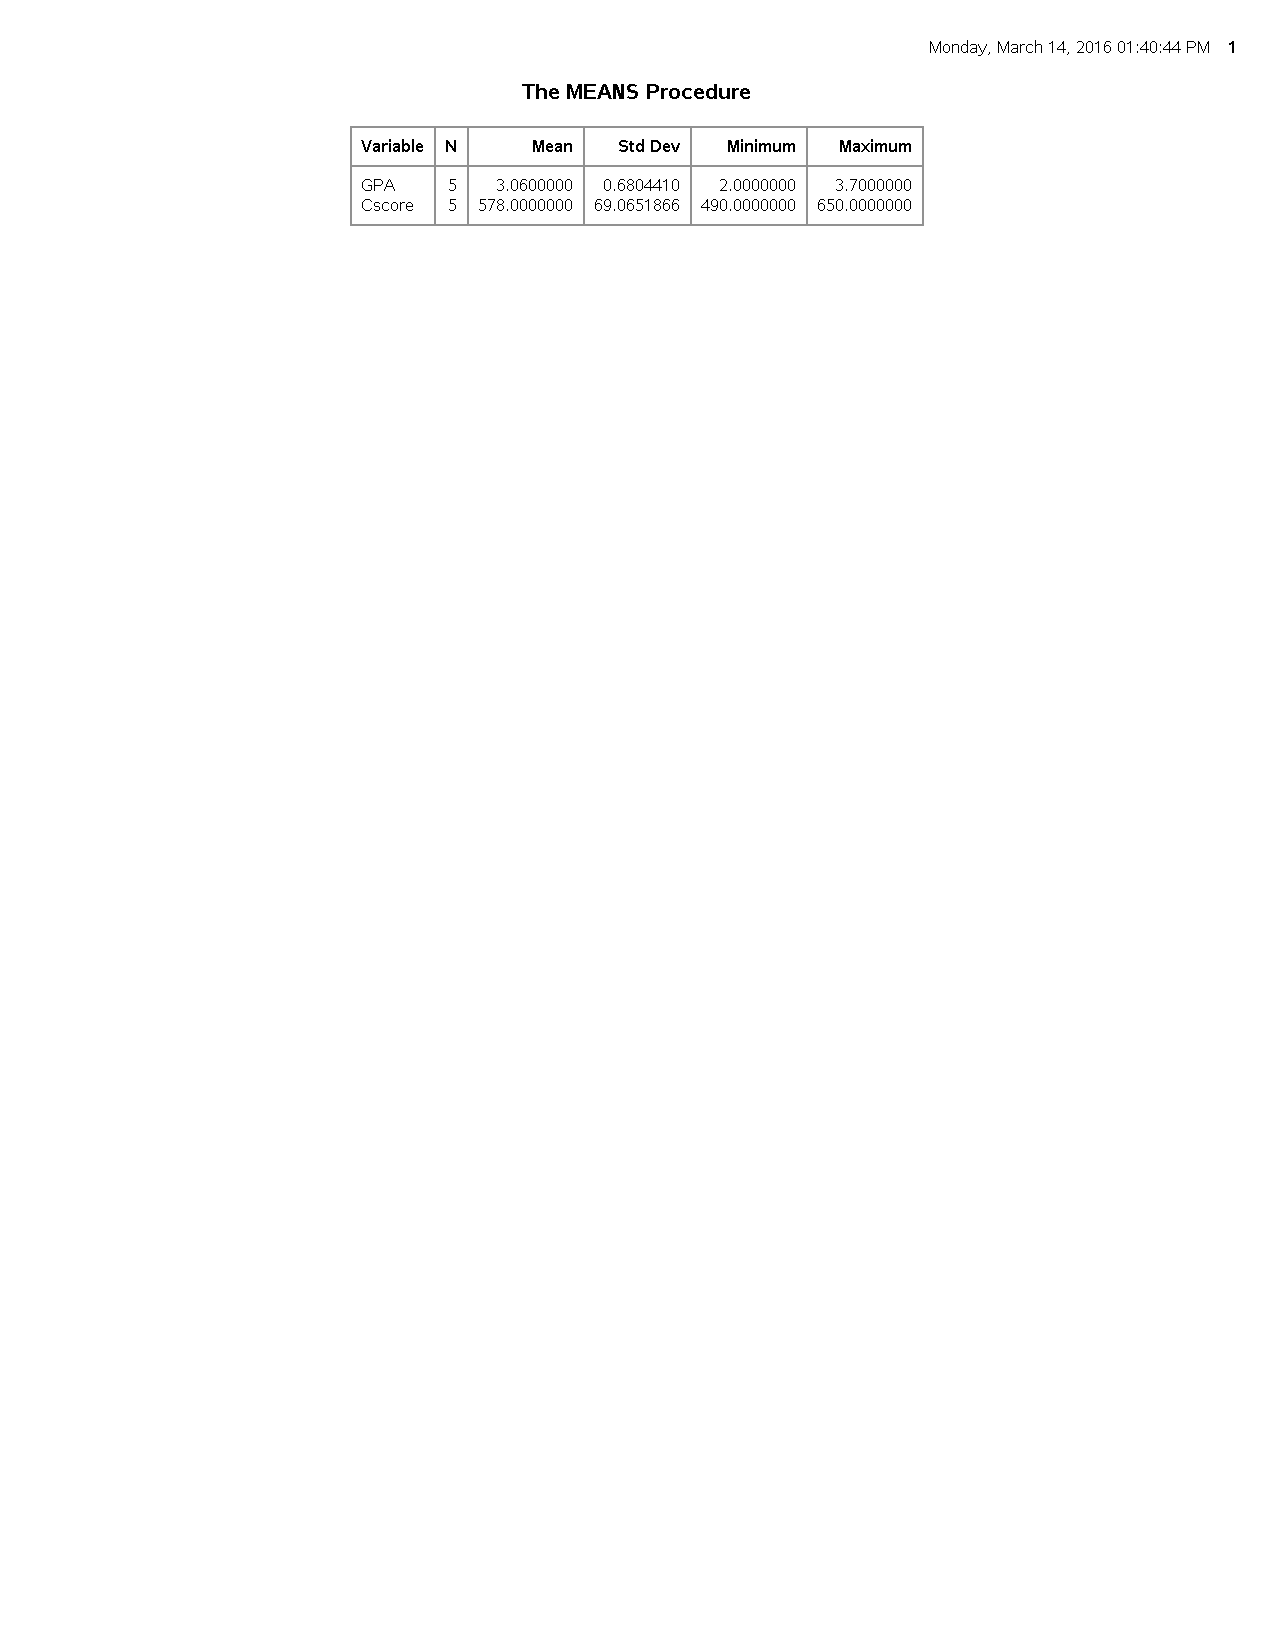
\includepdf{hw25_01.pdf}

\begin{Verbatim}
/* 2 */ 
DATA prob2;
	input SUBJ 1-3 
		  HEIGHT 4-5 
		  WT_INIT 6-8 
		  WT_FINAL 9-11;
	BMI_INIT = (WT_INIT / (2.2 * HEIGHT * 0.0254))*
			   (WT_INIT / (2.2 * HEIGHT * 0.0254));

	BMI_FINAL = (WT_FINAL / (2.2 * HEIGHT * 0.0254))*
				(WT_FINAL / (2.2 * HEIGHT * 0.0254));

	BMI_DIFF = BMI_FINAL - BMI_INIT;
DATALINES;
00768155150
00272250240
00563240200
00170345298
;
proc sort data=prob2;
	by SUBJ;
run;
proc print data=prob2;
	var SUBJ HEIGHT BMI_INIT BMI_FINAL BMI_DIFF;
run;
\end{Verbatim}

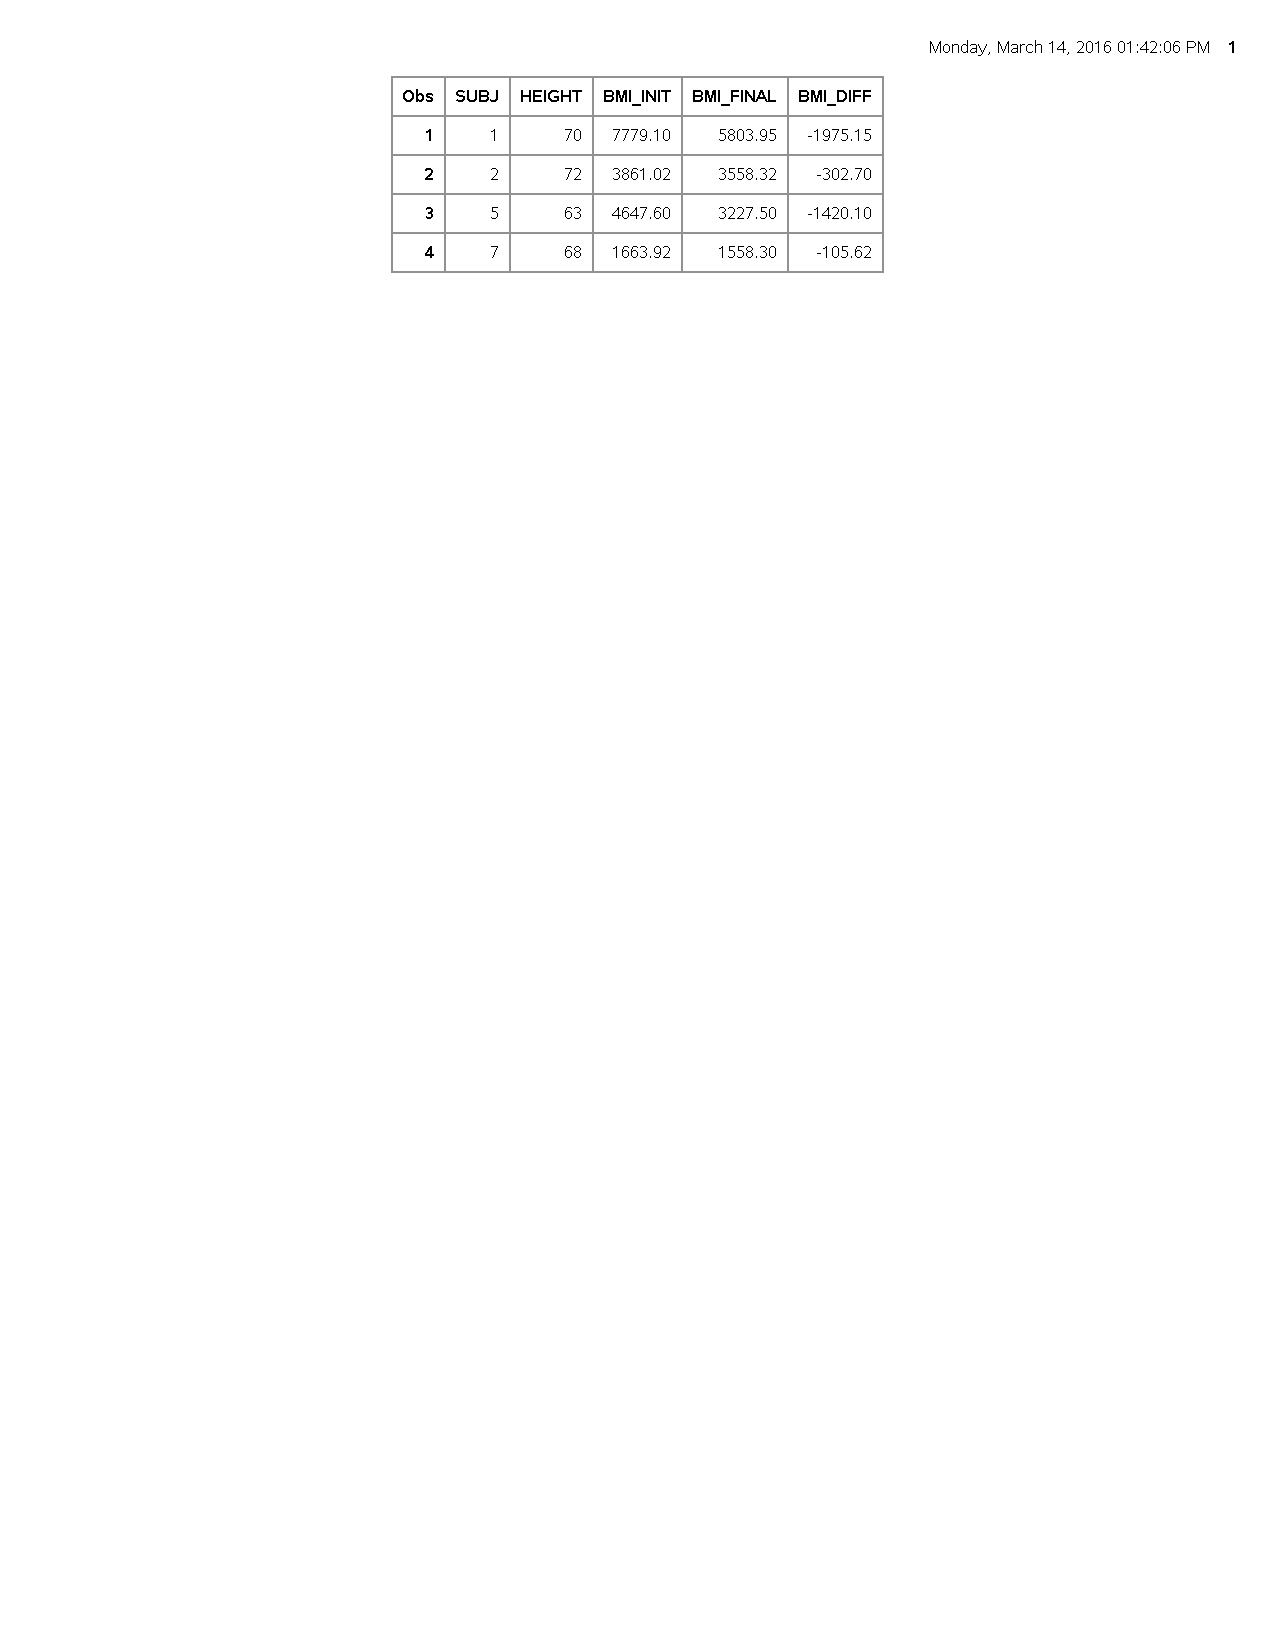
\includepdf{hw25_02.pdf}

\begin{Verbatim}
/* 3 */
DATA prob3;
	input SSN 1-9 salary 11-15 age 17-18 race $ 20;
	TAX = 0.3 * salary;
DATALINES;
123874414 28000 35 W
464239182 29500 37 B
012437652 35100 40 W
018451357 26500 31 W
;
proc means data=prob3;
	var salary age;
run;
proc sort data=prob3;
	by SSN;
run;
proc print data=prob3;
	var SSN salary TAX;
run;
\end{Verbatim}

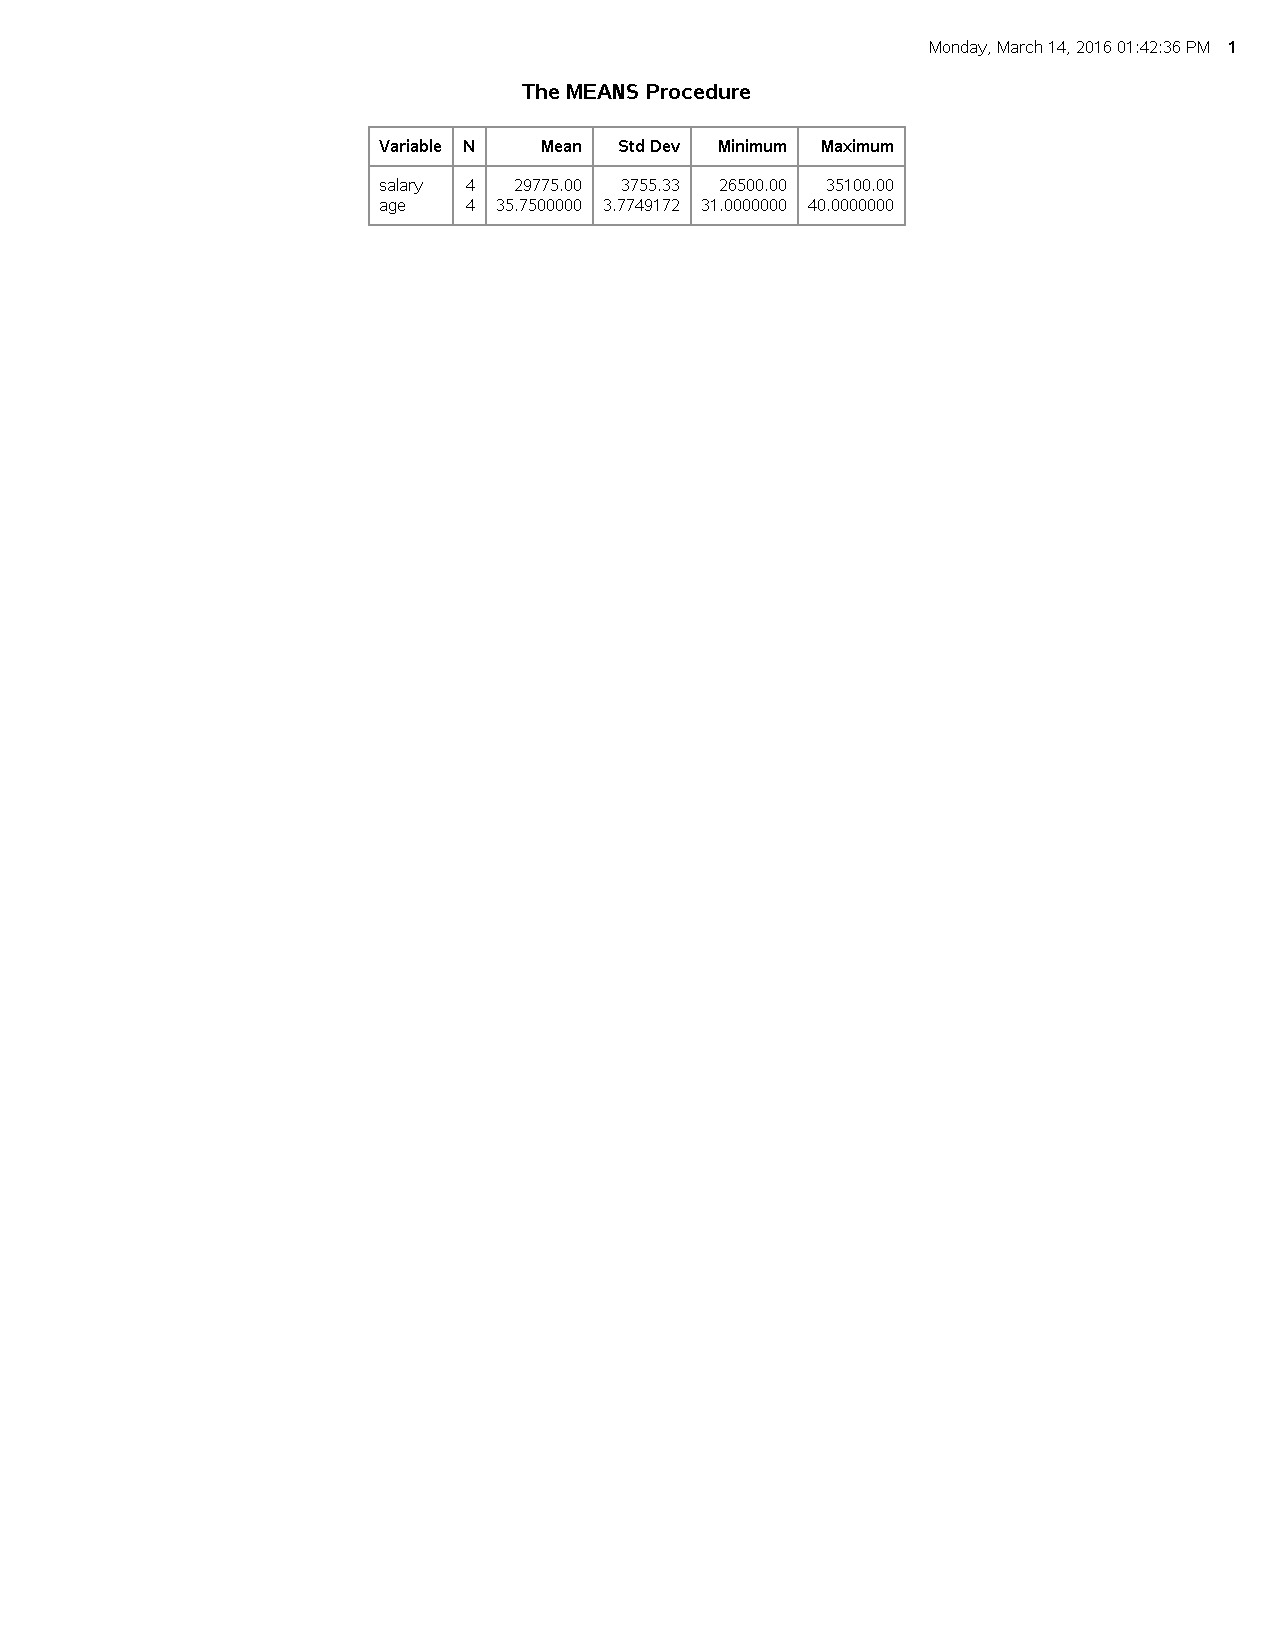
\includepdf{hw25_03.pdf}

\begin{Verbatim}
/* 4 */
DATA IQ_AND_TEST_SCORES;
	input ID 1-3
	      IQ 4-6
	      MATH 7-9
	      SCIENCE 10-12;
	OVERALL = (IQ + MATH + (SCIENCE / 500.0)) / 3.0;
	IF IQ GE 0 AND IQ LE 100 THEN GROUP = 1;
	ELSE IF IQ GT 100 AND IQ LE 140 THEN GROUP = 2;
	ELSE IF IQ GT 140 THEN GROUP = 3;
DATALINES;
001128550590
002102490501
003140670690
004115510510
;
proc sort data = IQ_AND_TEST_SCORES;
	by IQ;
run;
proc freq data = IQ_AND_TEST_SCORES;
	tables GROUP;
run;
\end{Verbatim}

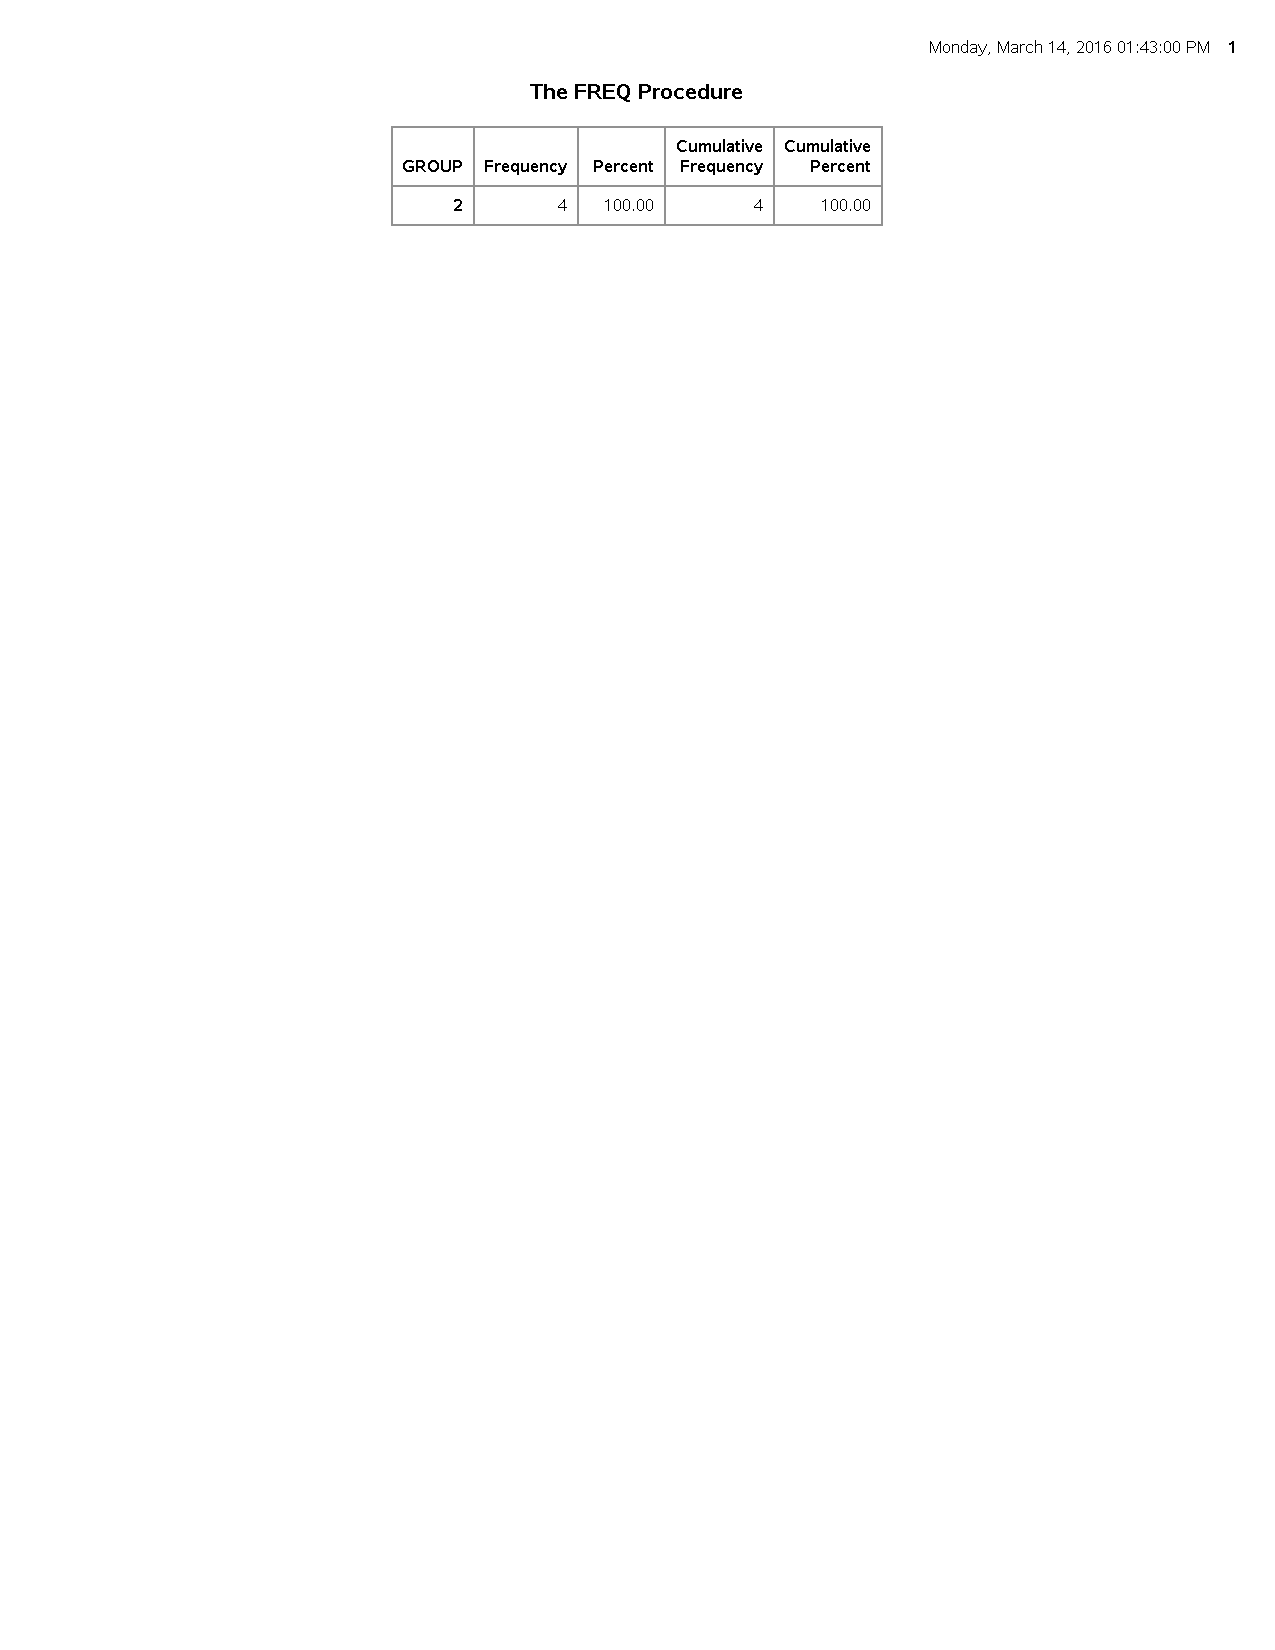
\includepdf{hw25_04.pdf}

\begin{Verbatim}
/* 5 */ 
**********************************************
The problem with the code for this example was 
Invalid Syntax on VOTER-TURNOUT
*********************************************;

/* 6 */
DATA SURVEY;
	input QUES1 $ 1 
	      QUES2 $ 2 
	      QUES3 $ 3 
	      QUES4 $ 4 
	      QUES5 $ 5;
DATALINES;
ABCDE
AACCE
BBBBB
CABDA
DDAAC
CABBB
EEBBB
ACACA
;
proc freq data = SURVEY;
	tables QUES1 QUES2 QUES3 QUES4 QUES5;
run;
\end{Verbatim}

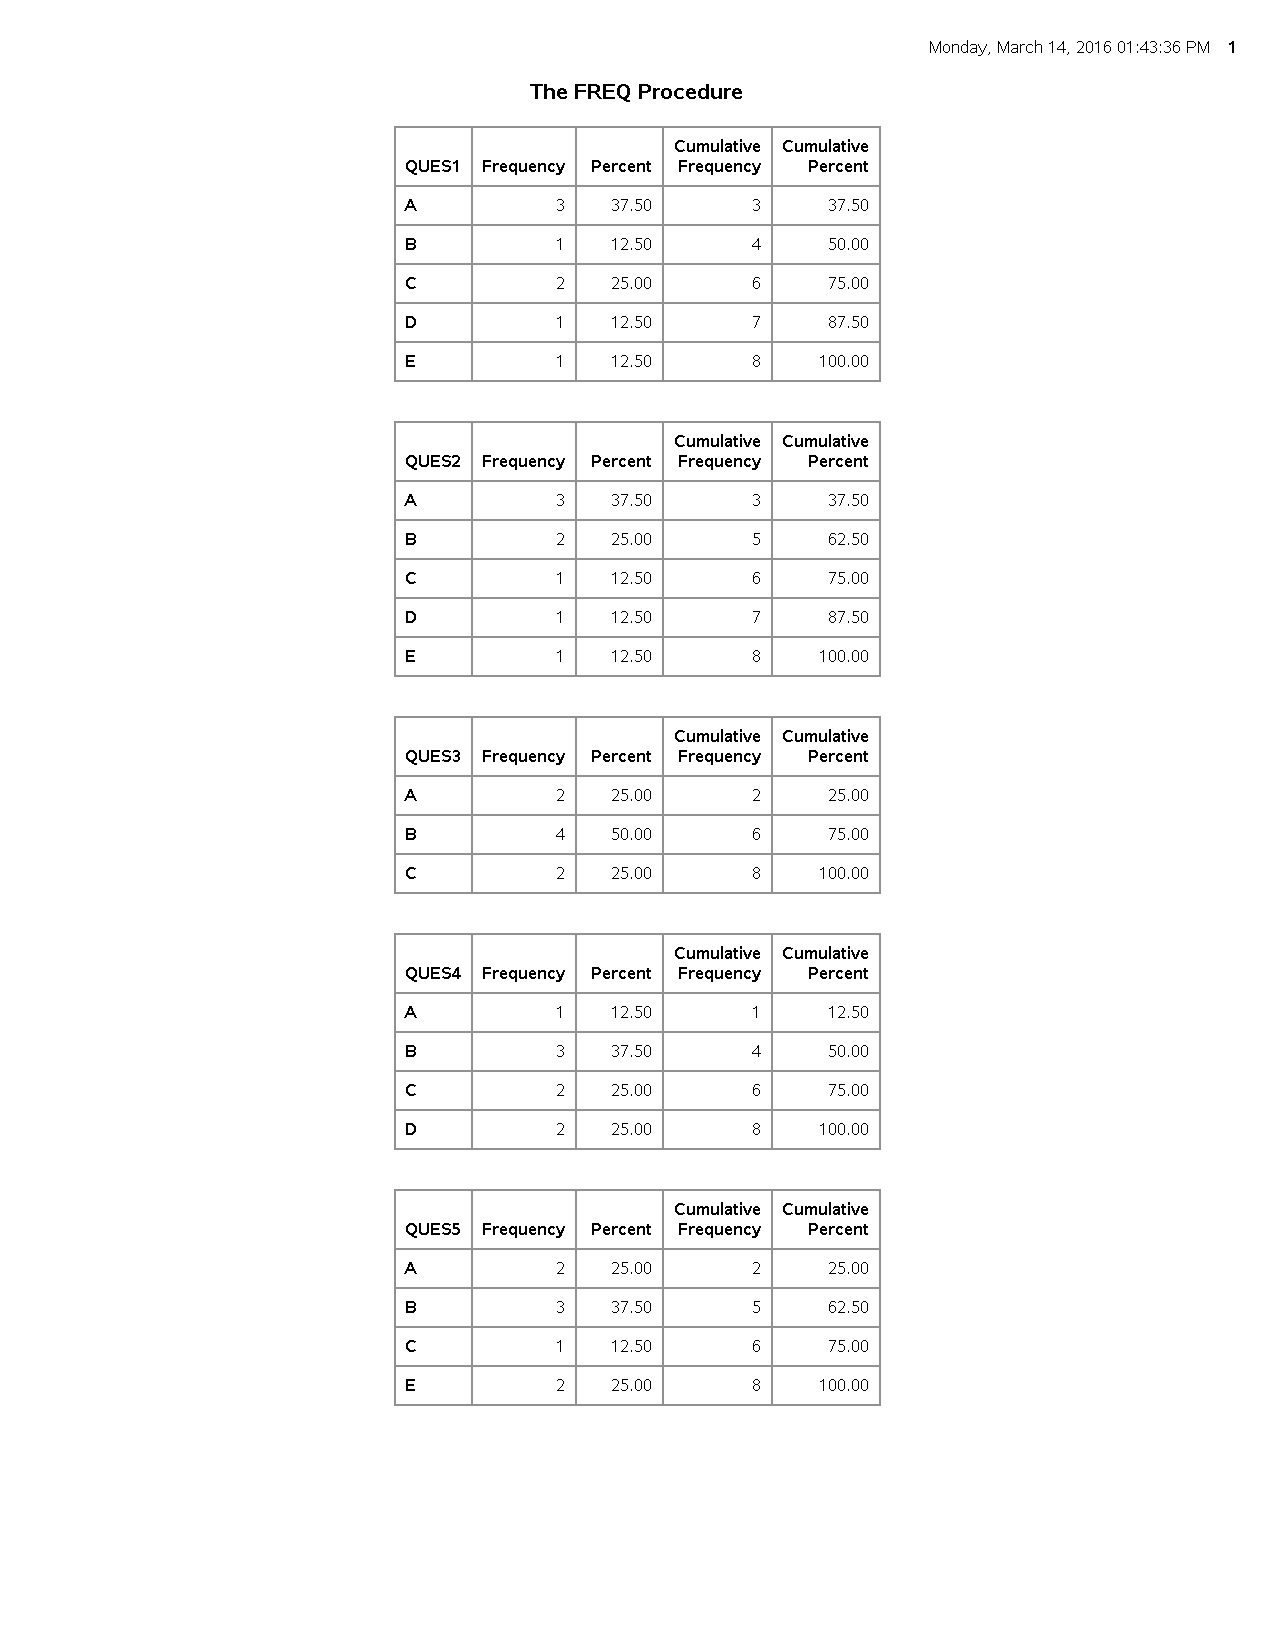
\includepdf{hw25_06.pdf}

\begin{Verbatim}
/* 7 */
data BUYER;
	input age 1-2
		  gender $ 3 
		  race $ 4 
		  income 5-10  
		  marital_status $ 11
		  own_home $ 12;
DATALINES;
;
proc means data=BUYER;
	var age gender income;
run;

/* 8 */
data EMPLOYEE;
	input EMPID
		  SALARY
		  JCLASS;
	IF JCLASS EQ 1 THEN BONUS = 0.1 * SALARY;
	ELSE IF JCLASS EQ 2 THEN BONUS = 0.15 * SALARY;
	ELSE IF JCLASS EQ 3 THEN BONUS = 0.2 * SALARY;
	NEW_SALARY = SALARY + BONUS;
datalines;
137 2800 1
214 9800 3
199 150000 3
355 57000 2
;
proc print data=EMPLOYEE;
run;
\end{Verbatim}

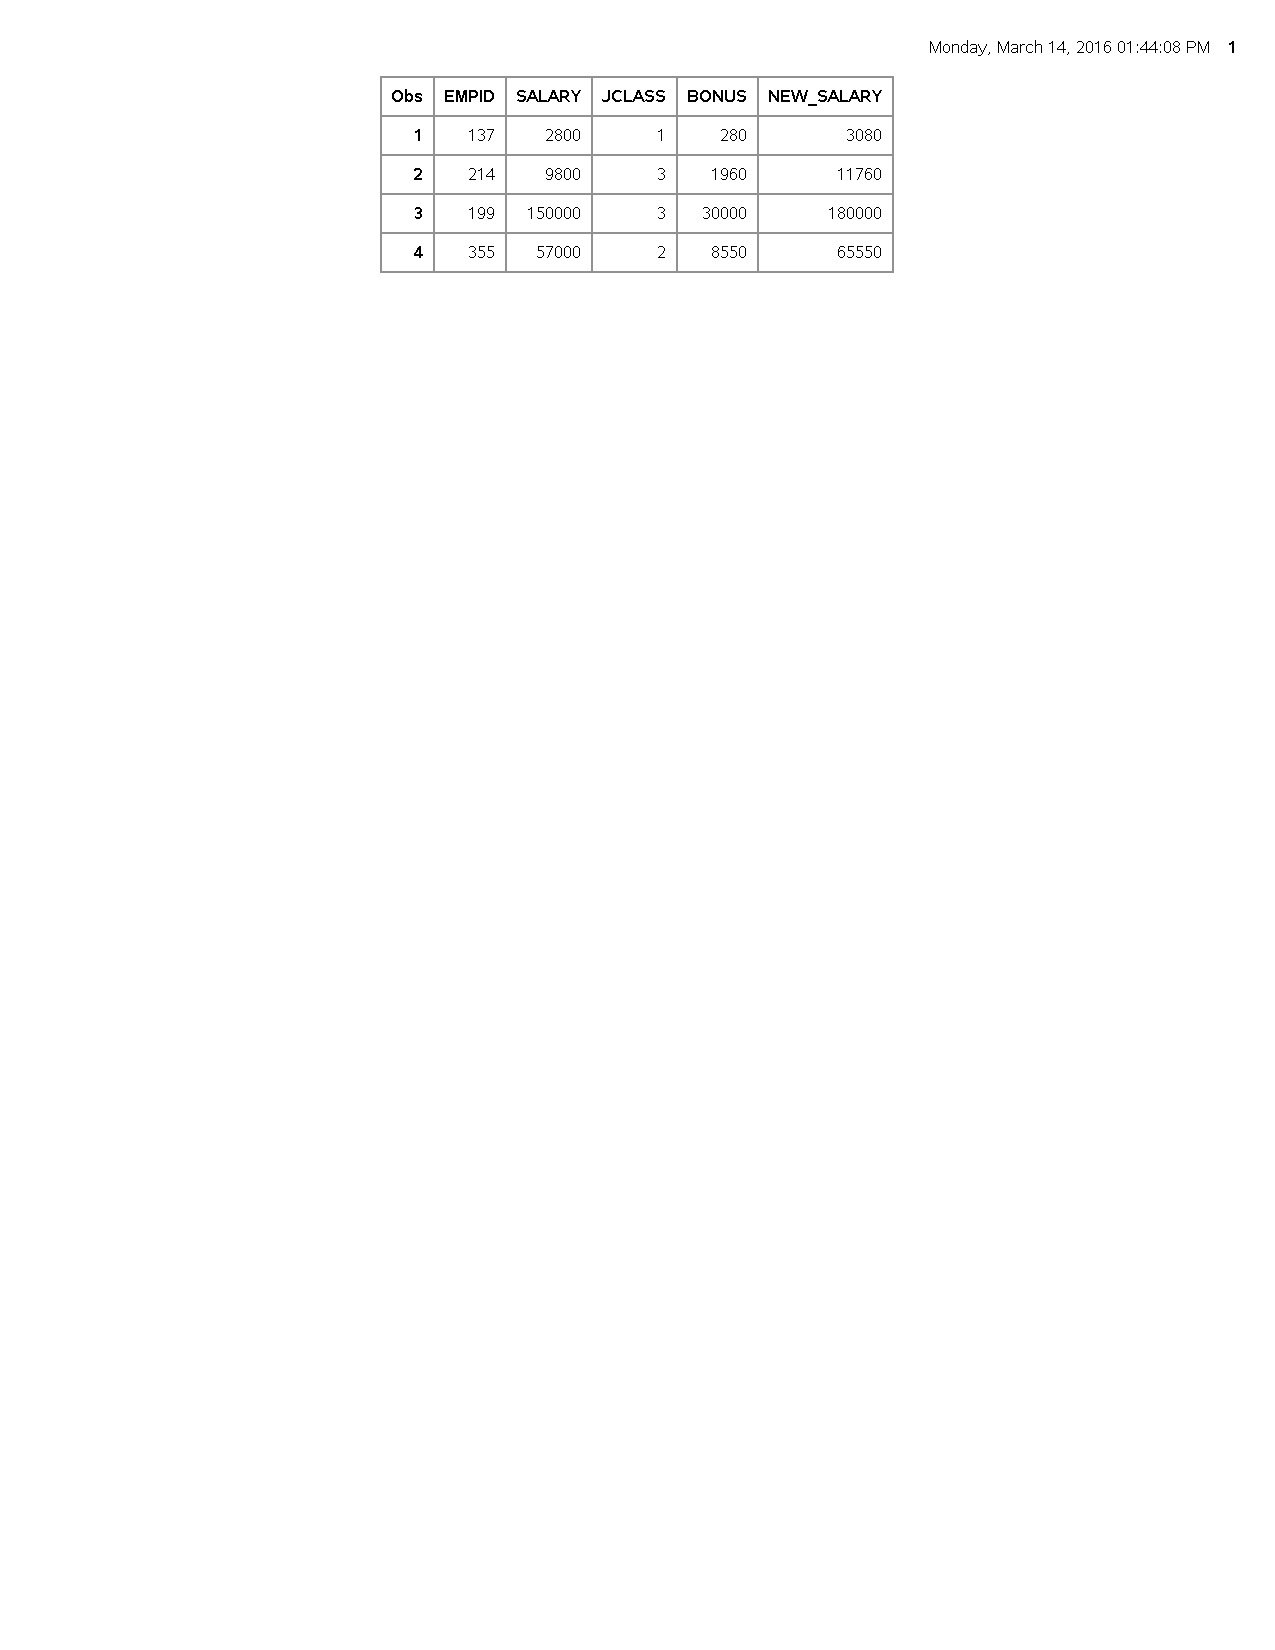
\includepdf{hw25_08.pdf}

\begin{Verbatim}
/* 9 */
data prob9; 
	input ID 1-3 RACE $ 4 SBP 5-7 DBP 8-9 HR 10-11;
datalines;
001W1308060
002B1409070
003W1207064
004W1509076
005B1248672
;
proc sort data=prob9;
	by SBP;
run;
proc print data = prob9 NOOBS;
	TITLE "RACE AND HEMODYNAMIC VARIABLES";
	var ID RACE SBP DBP;
run;
\end{Verbatim}

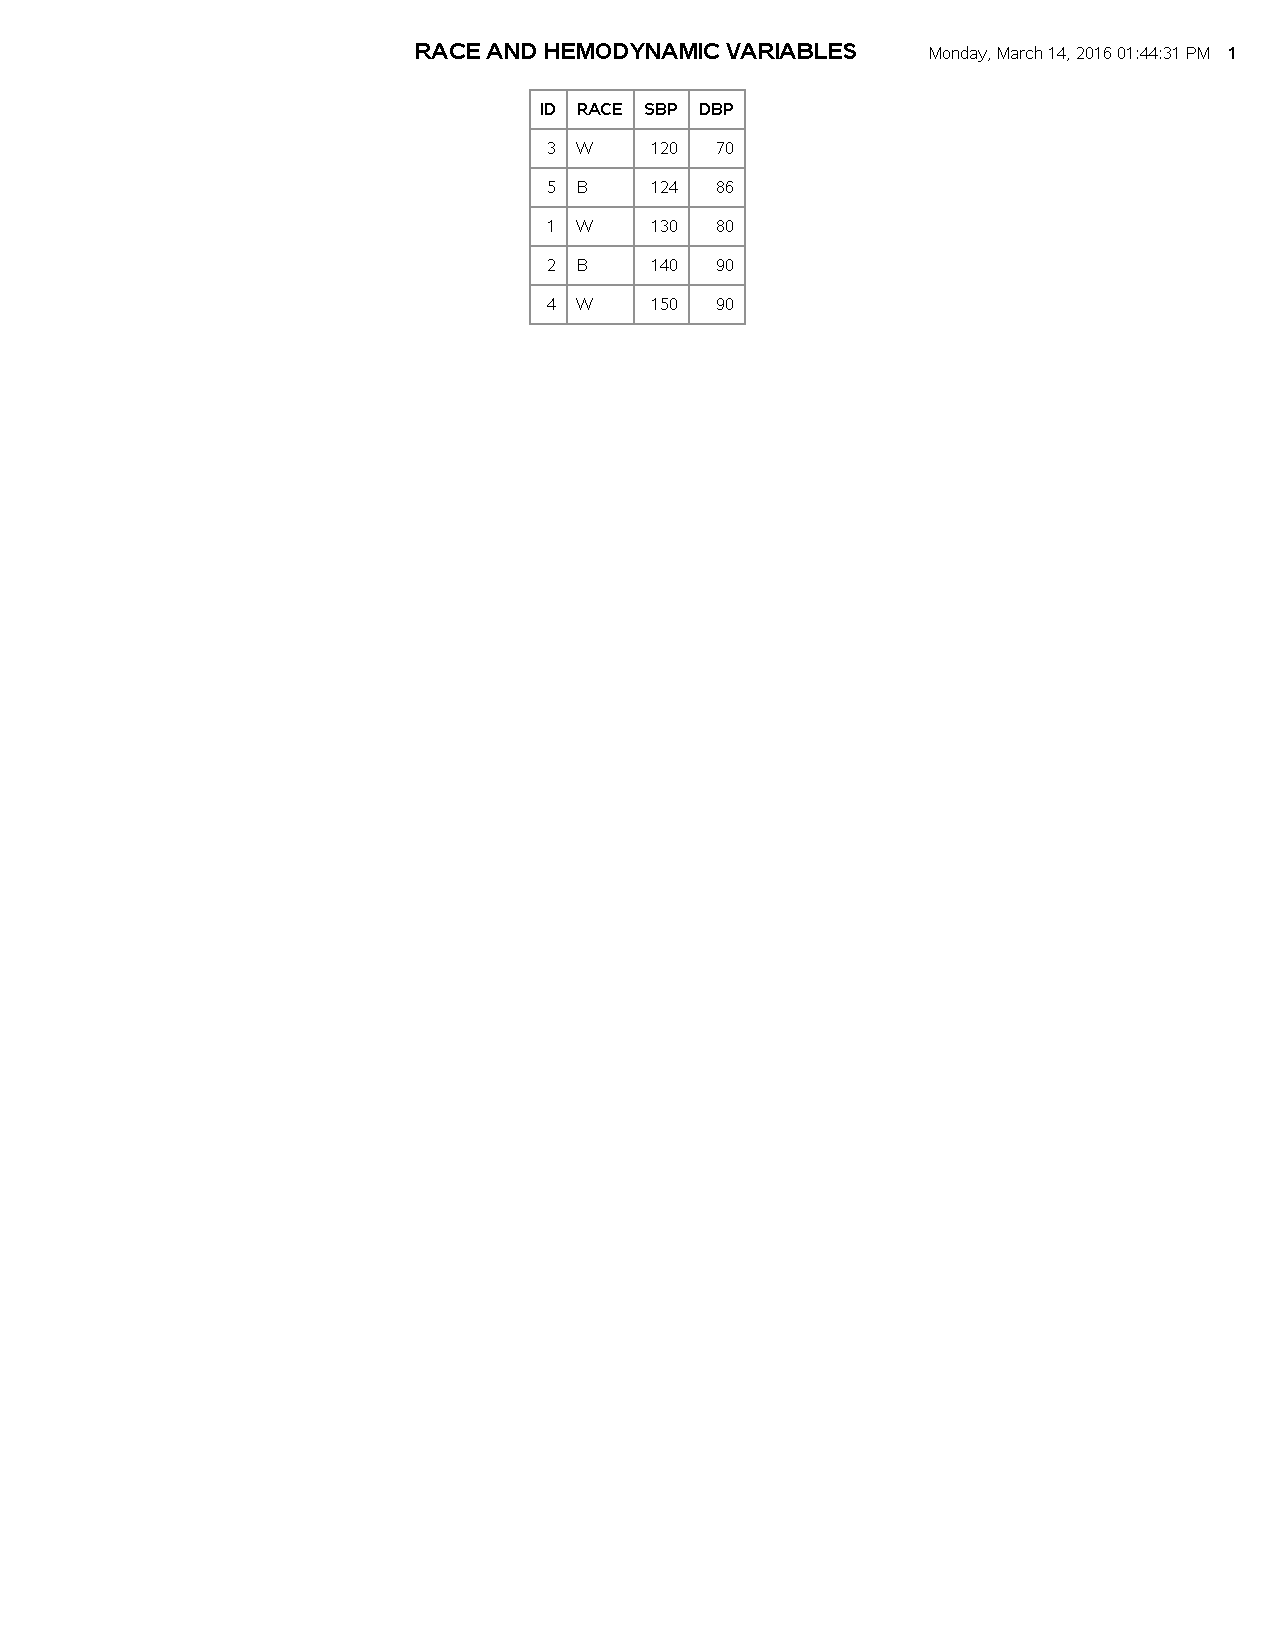
\includepdf{hw25_09.pdf}

\begin{Verbatim}
/* 10 */
data RAIN;
	input CITY $ 
		  RAIN_JUNE 
		  RAIN_JULY 
		  RAIN_AUGUST;
	AVERAGE = (RAIN_JUNE + RAIN_JULY + RAIN_AUGUST)/ 3.0;
	PERCENT_JUNE = 100 * RAIN_JUNE / AVERAGE;
	PERCENT_JULY = 100 * RAIN_JULY / AVERAGE;
	PERCENT_AUGUST = 100 * RAIN_AUGUST / AVERAGE;
datalines;
TRENTON 23 25 30
 NEWARK 18 27 22
 ALBANY 22 21 27
;
proc sort data=RAIN;
	by CITY;
run;
proc means maxdec=2 clm mean stddev alpha=0.05 data=RAIN;
	var RAIN_JUNE RAIN_JULY RAIN_AUGUST;
run;
\end{Verbatim}

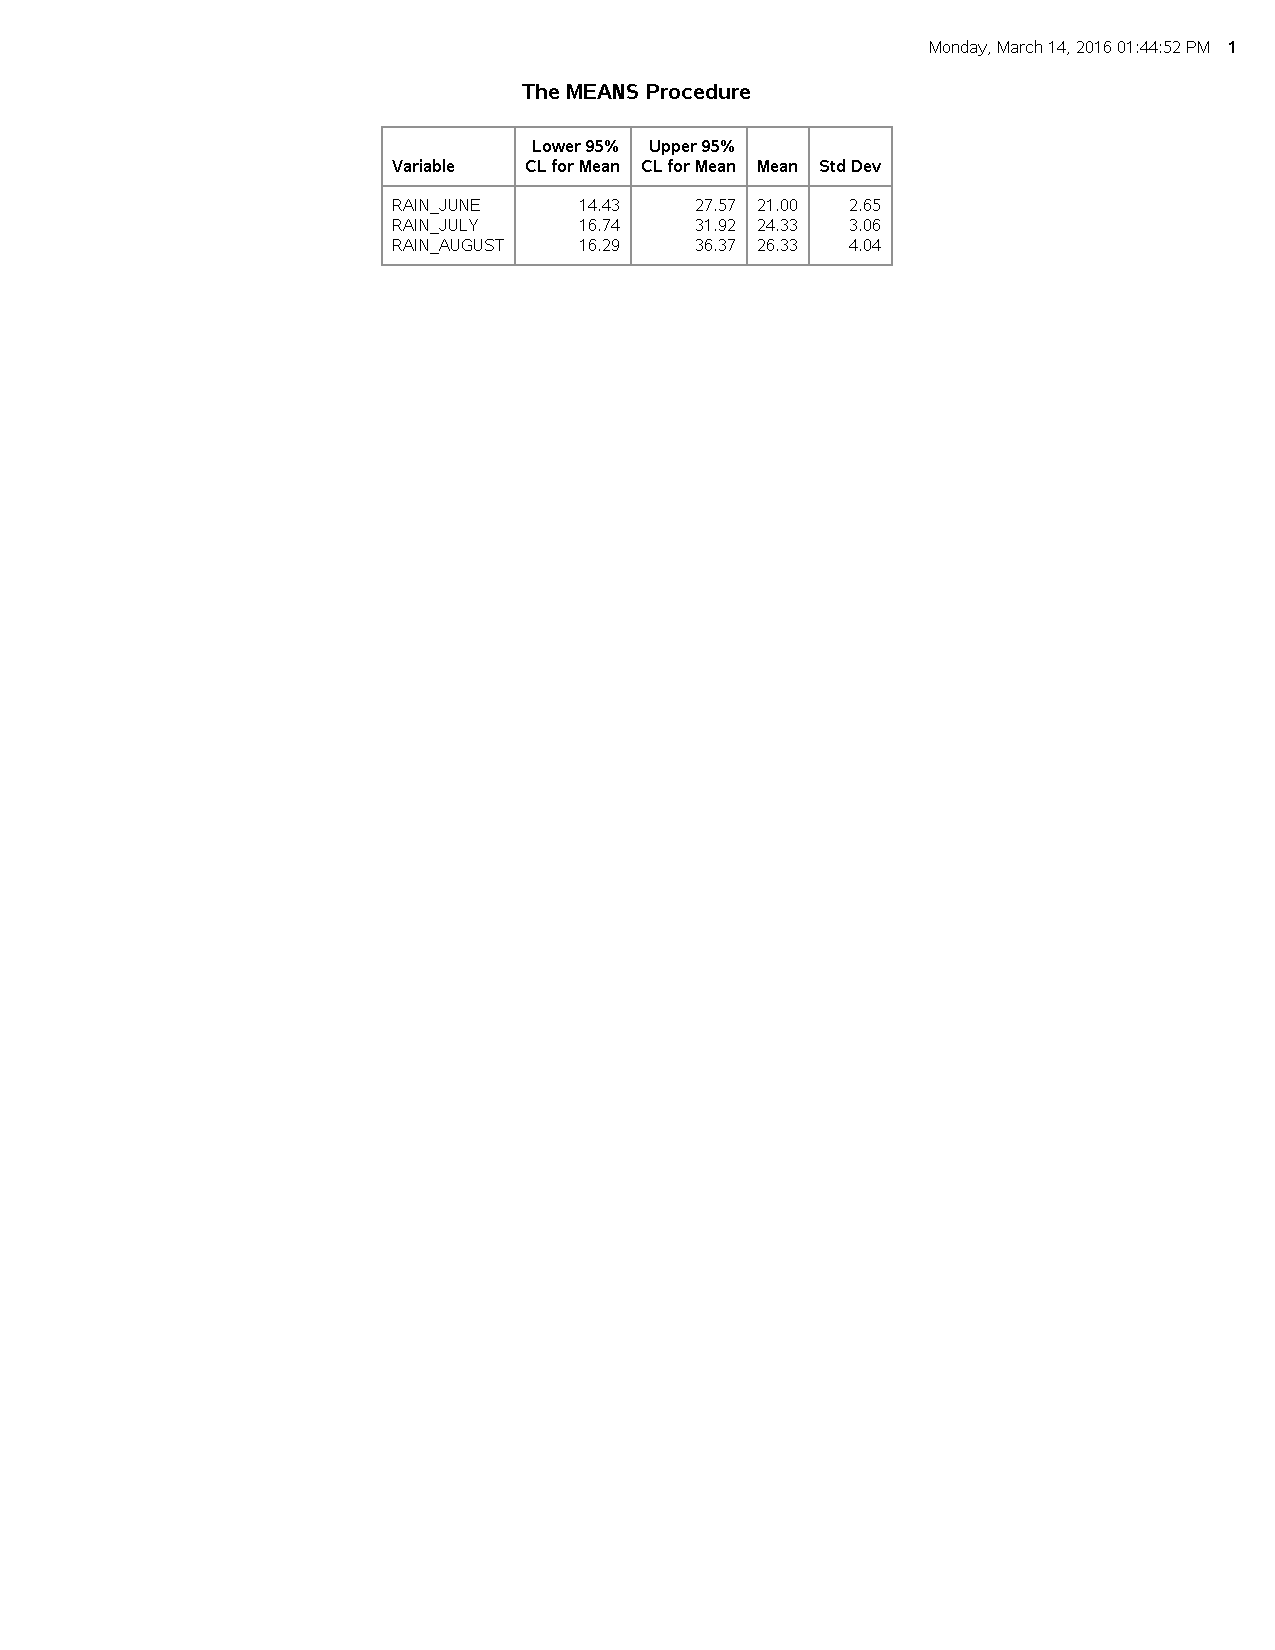
\includepdf{hw25_10.pdf}
\end{document}
